\chapter{Object Detection using Faster R--CNN}

\indent\indent Object detection is a computer vision task that involves predicting where the required objects are in an image. This chapter gives an introduction to object detection. It further gives details on one of the most efficient object detection algorithms, the Faster \acrshort{rcn} model and then gives the summary of the trained object detection model.  
\section{Introduction to Object Detection}
Image Processing is a technique that plays out a couple of assignments in a picture, to generate a picture which is improved or to extricate information that is supportive from it. A kind of sign handling it is, in which info is a picture and yield may be picture or highlights related with that image. In the recent days, image preparing is one of the rapidly creating developments. It shapes focus examine district inside structure and disciplines too of programming building. Picture handling incorporates fundamentally the three accompanying stages, bringing in the picture by means of securing picture instruments, controlling and breaking down the picture and yield in which the end data can be changed picture or report that depends on picture examination. There are couple of types of strategies used for picture preparing explicitly, simple and computerized image handling. Image specialists use few nuts and bolts of comprehension while simultaneously using these visual procedures. Advanced Image handling strategies help in charge of the modernized pictures by using PCs. A library fundamentally focused on current-time computer vision of programming capacities is \gls{ocv}. \gls{ocv} bolsters a few models from profound learning structures like TensorFlow, Torch, PyTorch (subsequent to changing over to an ONNX model) and Caffe as indicated by a characterized rundown of upheld layers. It
advances OpenVisionCapsules, which is a versatile configuration, perfect with every other arrangement.\\
Computer vision is an interdisciplinary field that has been gaining huge amounts of traction in the recent years(since CNN) and self-driving cars have taken centre stage. Another integral part of computer vision is object detection. Object detection aids in pose estimation, vehicle detection, surveillance etc. The difference between object detection algorithms and classification algorithms is that in detection algorithms, we try to draw a bounding box around the object of interest to locate it within the image. Also, you might not necessarily draw just one bounding box in an object detection case, there could be many bounding boxes representing different objects of interest within the image and you would not know how many beforehand.\\
Object detection \cite{8627998} is a computer vision technique which used image processing that allows us to identify and locate objects in an image or video. With this kind of identification and localization, object detection can be used to count objects in a scene and determine and track their precise locations, all while accurately labeling them.\\
Object recognition is a general term to describe a collection of related computer vision tasks that involve identifying objects in digital photographs.
Image classification involves predicting the class of one object in an image. Object localization refers to identifying the location of one or more objects in an image and drawing abounding box around their extent. Object detection combines these two tasks and localizes and classifies one or more objects in an image.\\
As such, we can distinguish between these three computer vision tasks:
\begin{enumerate}
\item Image Classification: Predict the type or class of an object in an image.
\begin{enumerate}
    \item Input: An image with a single object, such as a photograph.
    \item Output: A class label (e.g. one or more integers that are mapped to class labels).
\end{enumerate}
\item Object Localization: Locate the presence of objects in an image and indicate their location with a bounding box.
\begin{enumerate}
    \item Input: An image with one or more objects, such as a photograph.
    \item Output: One or more bounding boxes (e.g. defined by a point, width, and height).
\end{enumerate}
\item Object Detection: Locate the presence of objects with a bounding box and types or classes of the located objects in an image.
\begin{enumerate}
    \item Input: An image with one or more objects, such as a photograph.
    \item Output: One or more bounding boxes (e.g. defined by a point, width, and height), and a class label for each bounding box.
\end{enumerate}
\end{enumerate}
% \ref{fig:object} 
\begin{figure}[H]
\centering
	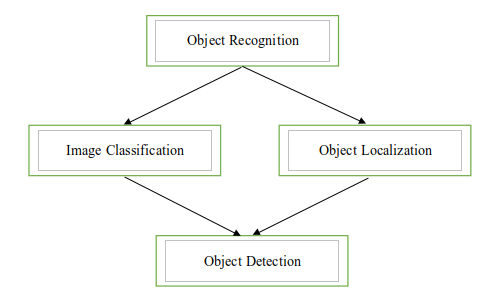
\includegraphics[scale=1]{Figures/object.png}	
	\caption{Object Detection}
	\label{fig:object}
\end{figure}
A naive approach to solve this problem would be to take different regions of interest from the image, and use a CNN to classify the presence of the object within that region. The problem with this approach is that the objects of interest might have different spatial locations within the image and different aspect ratios. Hence, you would have to select a huge number of regions and this could computationally blow up. Therefore, algorithms like \acrshort{rcn}, YOLO etc have been developed to find these occurrences and find them fast.
\section{Introduction to \acrlong{rcn}}
The problem the R--CNN system tries to solve it is to locate objects in an image (object detection). R--CNN “Region-based Convolutional Neural Networks”. The main idea is composed of two steps. 
\begin{enumerate}
    \item First, using selective search, it identifies a manageable number of bounding-box object region candidates (“region of interest” or “RoI”). 
    \item It then extracts CNN features from each region independently for classification.
\end{enumerate}
To make \acrshort{rcn} faster, the training procedure was improved by unifying three independent models into one jointly trained framework and increasing shared computation results, named Fast \acrshort{rcn}. Instead of extracting CNN feature vectors independently for each region proposal, this model aggregates them into one CNN forward pass over the entire image and the region proposals share this feature matrix. Then the same feature matrix is branched out to be used for learning the object classifier and the bounding-box regressor. In conclusion, computation sharing speeds up \acrshort{rcn}. Fast \acrshort{rcn} is much faster in both training and testing time. However, the improvement is not dramatic because the region proposals are generated separately by another model and that is very expensive.\\
An intuitive speedup solution is to integrate the region proposal algorithm into the CNN model. \acrlong{rcn} \cite{wang2017scene} is doing exactly this: construct a single, unified model composed of RPN (region proposal network) and fast R-CNN with shared convolutional feature layers.\\
\acrfull{rcn} is composed of 3 neural networks — Feature Network, Region Proposal Network (RPN), Detection Network.

\section{Software Setup}
\begin{enumerate}
\item Tensorflow: It is an open source stage from start to finish for AI. An exhaustive, biological system of instruments that is adaptable is included in it, network assets and libraries that lets ML to be pushed best in class by scientist and ML fueled applications are effectively assembled and conveyed by engineers.
\item LabelImg tool: LabelImg is a free, open source tool for graphically labeling images. It's written in Python and uses QT for its graphical interface. It is an 
an open-source image labeling tool for training classifiers.
\end{enumerate}

\section{Text Detection model using \acrlong{rcn}}
The object detection was successfully performed using TensorFlow object detection. COCO models provided pre-defined models for object detection. A variety of models with pre-assigned set of initial weights and pre-made architectures allowed flexibility in choosing the models based on training results. The faster{\_}rcnn{\_}v2{\_}coco model \cite{bhat2018cost} offered a considerably greater accuracy. Here the \acrshort{rcn} \cite{8627998} model applies high-capacity convolutional neural networks so that a fixed-length feature vector from each region can be extracted which is then fed to a set of class-specific linear SVMs. The Fast \acrshort{rcn} and \acrlong{rcn} \cite{wang2017scene} have made further evolution on the pipeline of object detection. Following the pioneering \acrshort{rcn}, Fast/Faster \acrshort{rcn} uses convolutional layers, initialized with discriminative pretraining for ImageNet classification, to extract region-independent features followed by a region wise multilayer perceptron (MLP) for classification. Datasets were made using LabelImg, an open-source image labeling tool for training classifiers. \\
The faster{\_}rcnn{\_}inception{\_}v2{\_}coco provides a special inception block to reduce the feature map size. These size reduction blocks have parameters specifically to maintain alignment of the feature map size in the concatenation layer.\\
% \ref{fig:object_summ} 
\begin{figure}[H]
\centering
	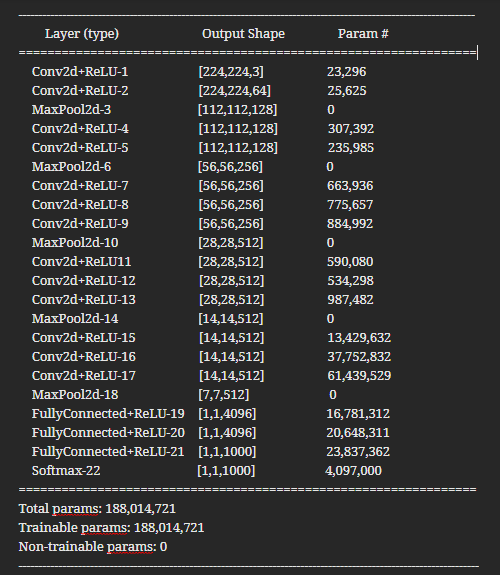
\includegraphics[scale=0.7]{Figures/object_summ.png}	
	\caption{Model summary of the text detection model}
	\label{fig:object_summ}
\end{figure}


\vspace{0.75cm}
 In  this chapter we saw that \acrlong{rcn} is faster in both training and testing and is much more efficient than the traditional methods like CNN (Convolutional Neural Networks) and OCR (Optical Character Recognition) for object detection and also the details of the model used to build the text detector.
